% ------------------------------------------------------------------------
% ------------------------------------------------------------------------
% ------------------------------------------------------------------------
%                                Cap�tulo 2
% ------------------------------------------------------------------------
% ------------------------------------------------------------------------
% ------------------------------------------------------------------------

\chapter{Estado del arte}
% ------------------------------------------------------------------------
\noindent Es importante tener en cuenta los aportes que han hecho otros colegas en trabajos relacionados con el presente trabajo de grado, y por lo tanto, se har� referencia a algunos de estos proyectos. \\

Administraci�n de prototipo infraestructura de computaci�n en la nube del conuss con �nfasis en la implementaci�n de nuevos m�dulos de Openstack. Este trabajo tenia como objetivo administrar, monitorear y mantener el funcionamiento de la infraestructura de computaci�n en la nube modelo de alta disponibilidad del conuss, con �nfasis en la exploraci�n de nuevas tecnolog�as y otros m�dulos de Openstack en el conuss \citep{ThesisUis1}. \\

Estudio  de  una  alternativa  de  integraci�n  continua  que soporte  el  desarrollo  de  una infraestructura TI de  servicios  de informaci�n del transporte p�blico de pasajeros. Este trabajo tenia como objetivo dise�ar  y  evaluar  una  alternativa  de  integraci�n  continua  para  el desarrollo  de  los componentes de una infraestructura TI que ofrece servicios de informaci�n al transporte p�blico de pasajeros \citep{ThesisUis2}. \\

Implementaci�n de una nueva infraestructura de computaci�n en la nube con modelo de alta disponibilidad basada en Openstack y contenedores para el conuss. Este trabajo tenia como objetivo investigar y complementar el trabajo hecho previamente \citep{ThesisUis1} en conuss en la creaci�n de una infraestructura de nube \citep{ThesisUis3}. \\

Despliegue y monitorizaci�n de un cl�ster Mesos. Este trabajo tenia como finalidad utilizar un sistema de gesti�n de recursos en un conjunto de nodos computacionales (Mesos) para el despliegue y evaluaci�n del rendimiento de un cluster aplicaciones con diferentes complejidades algor�tmica \citep{thesisValencia}. \\

Despliegue de una aplicaci�n usando Docker y Kubernetes. Este trabajo tenia como finalidad de optimizar el proceso de despliegue de una aplicaci�n desarrollada por Sparta Consulting Ltd en un servidor con Minikube \citep{thesisOulun}. \\

Dise�o de una arquitectura cloud para una aplicaci�n con varios usuarios. Este trabajo tenia como finalidad dise�ar una arquitectura cloud que pudiera soportar una cantidad masiva de usuarios de una aplicaci�n de pagos m�vil \citep{thesisMath}. 


A su vez, existen arquitecturas cloud empresariales que pueden ser adaptadas seg�n los requerimientos del proyecto a implementar. \\

AWS provee un conjunto de servicios y cada arquitecto arma su arquitectura seg�n los requerimientos del proyecto y los servicios que proporciona AWS como podemos ver en la figura \ref{Arquitectura sugerida por AWS para una aplicaci�n en WordPress}. Este modelo es tambi�n utilizado por Microsoft Azure (Figura \ref{Arquitecturas sugeridas por Azure para una estaci�n de Blockchain}) y GCP(Figura \ref{Arquitecturas sugeridas por GCP para una aplicaci�n basada en eventos}). \\


\begin{figure}[h]
	\centering
	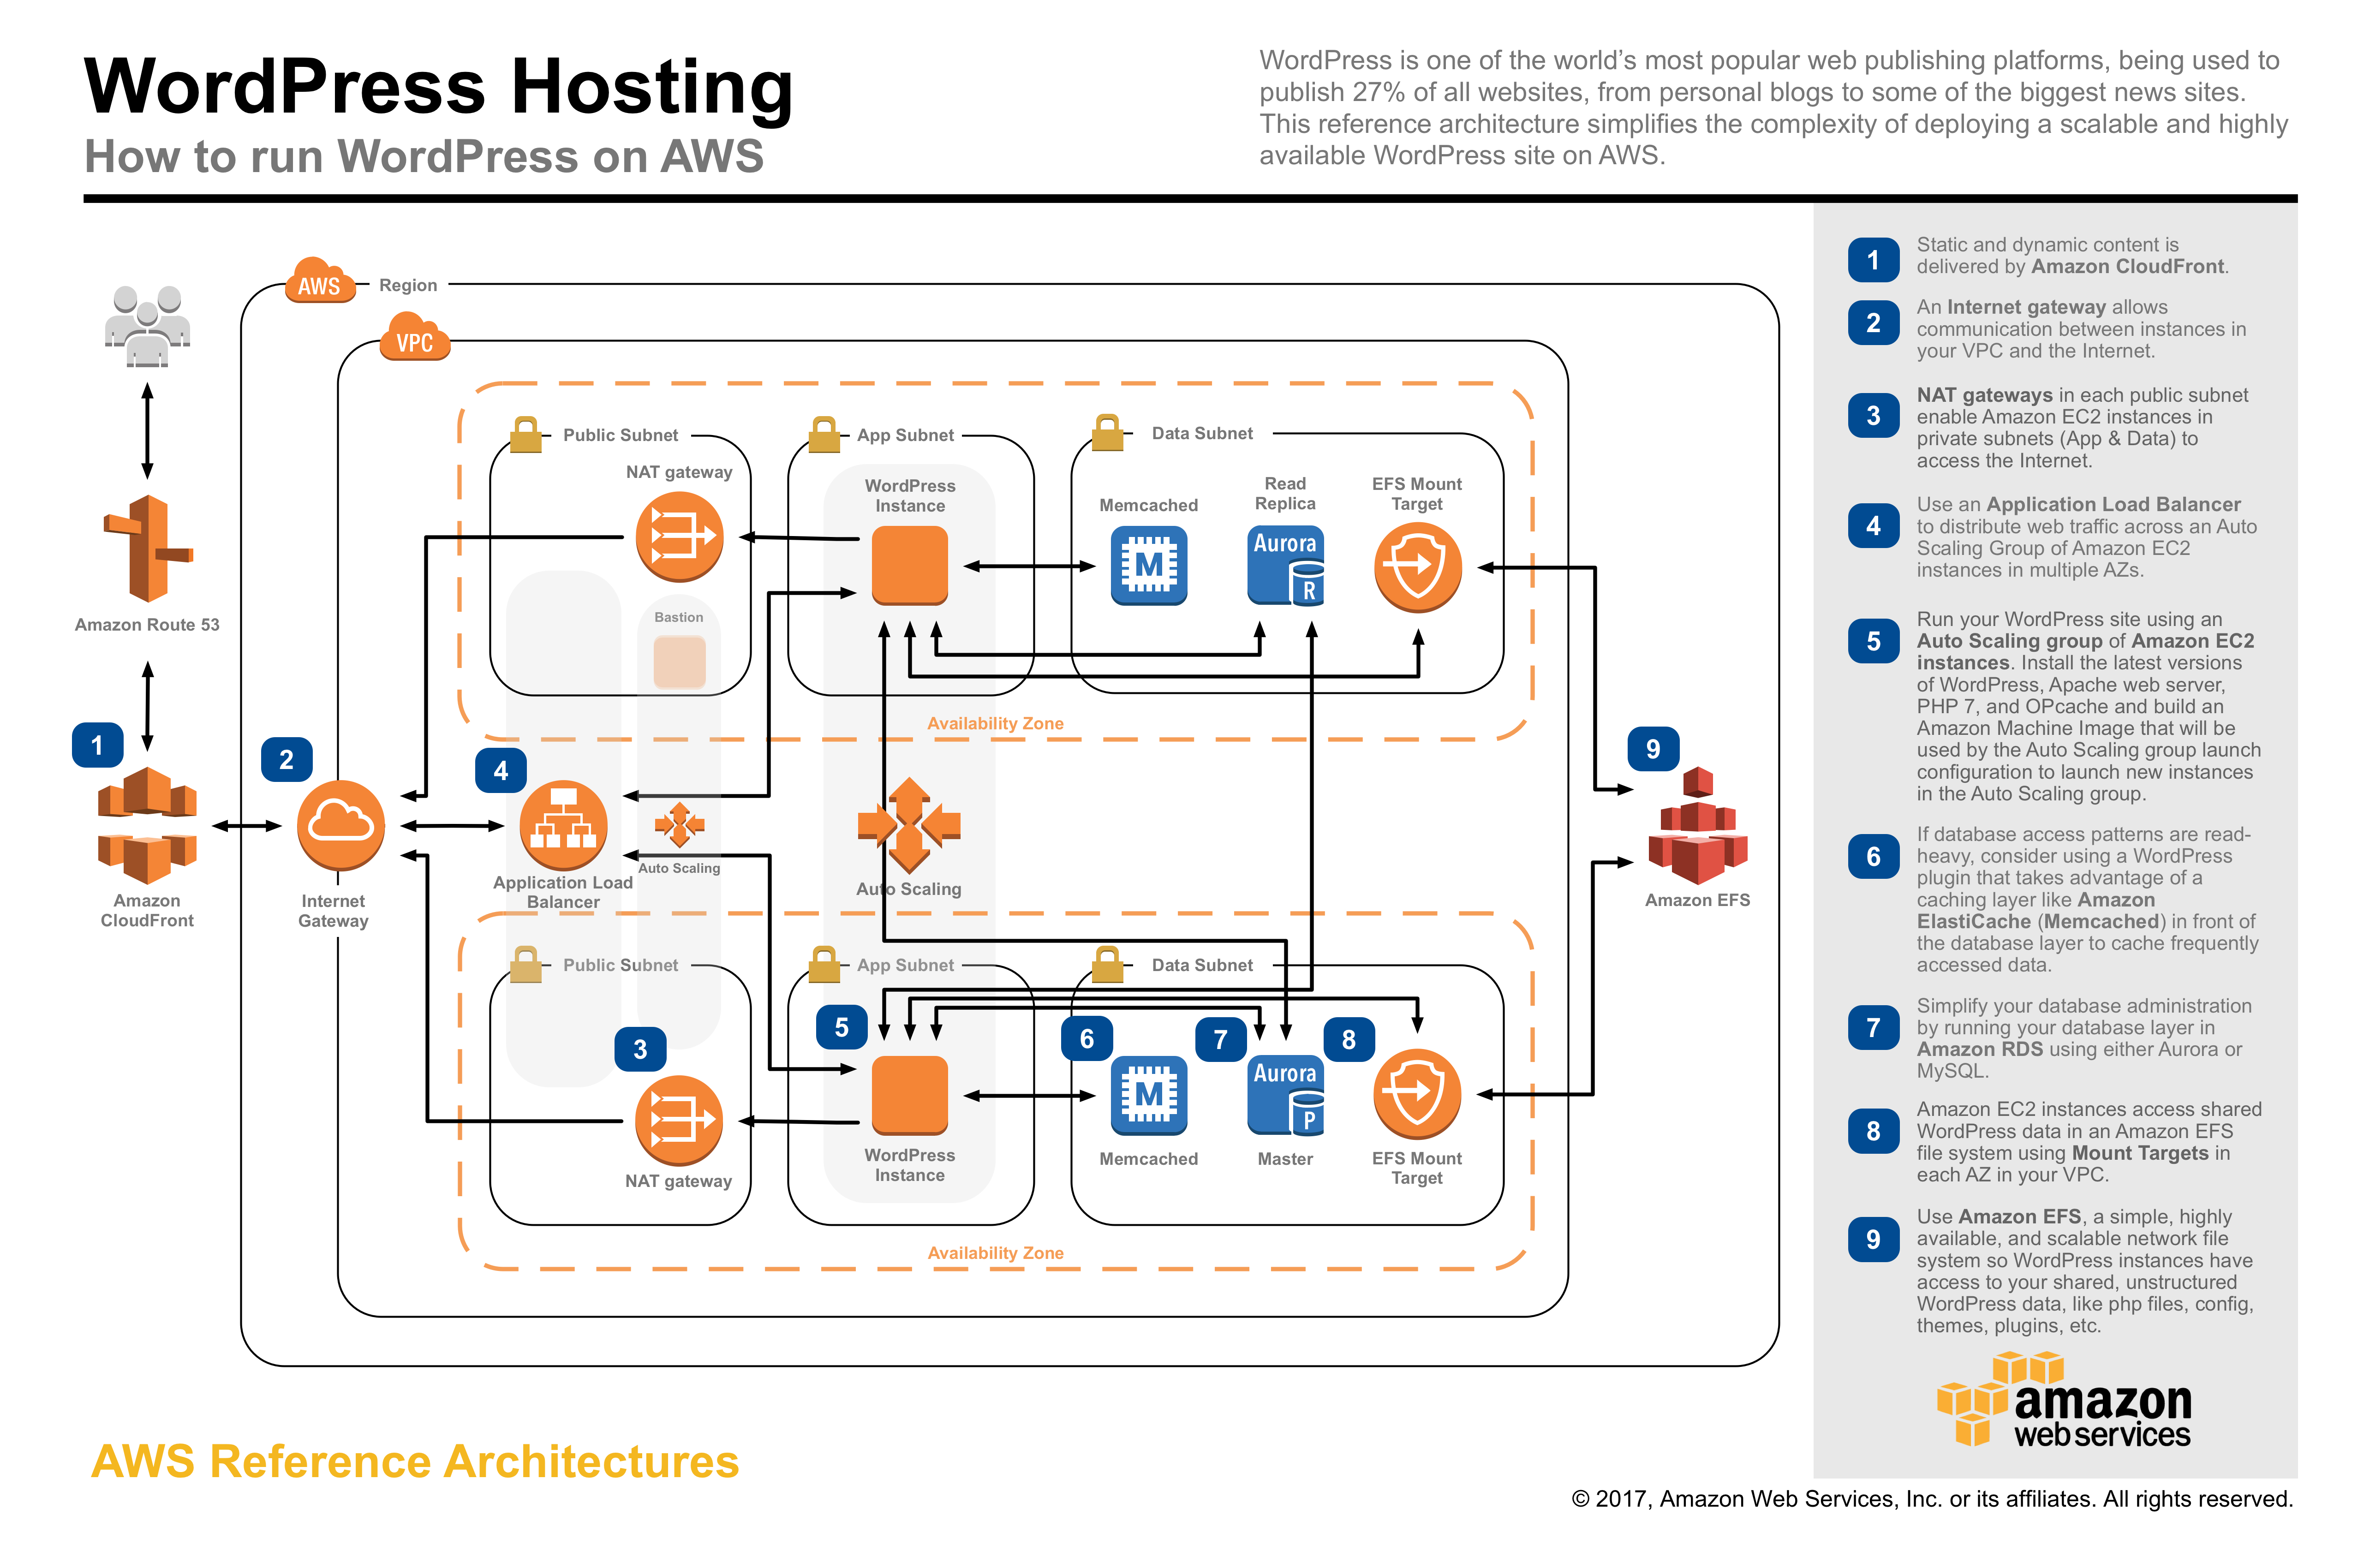
\includegraphics[width=0.75\textwidth]{figs/AWS_Arquitecturas.jpeg}
	\caption{Arquitectura sugerida por AWS para una aplicaci�n en WordPress. Adaptado de \citep{AwsArchitectureSample}}\label{Arquitectura sugerida por AWS para una aplicaci�n en WordPress}
\end{figure}

\begin{figure}[h]
	\centering
	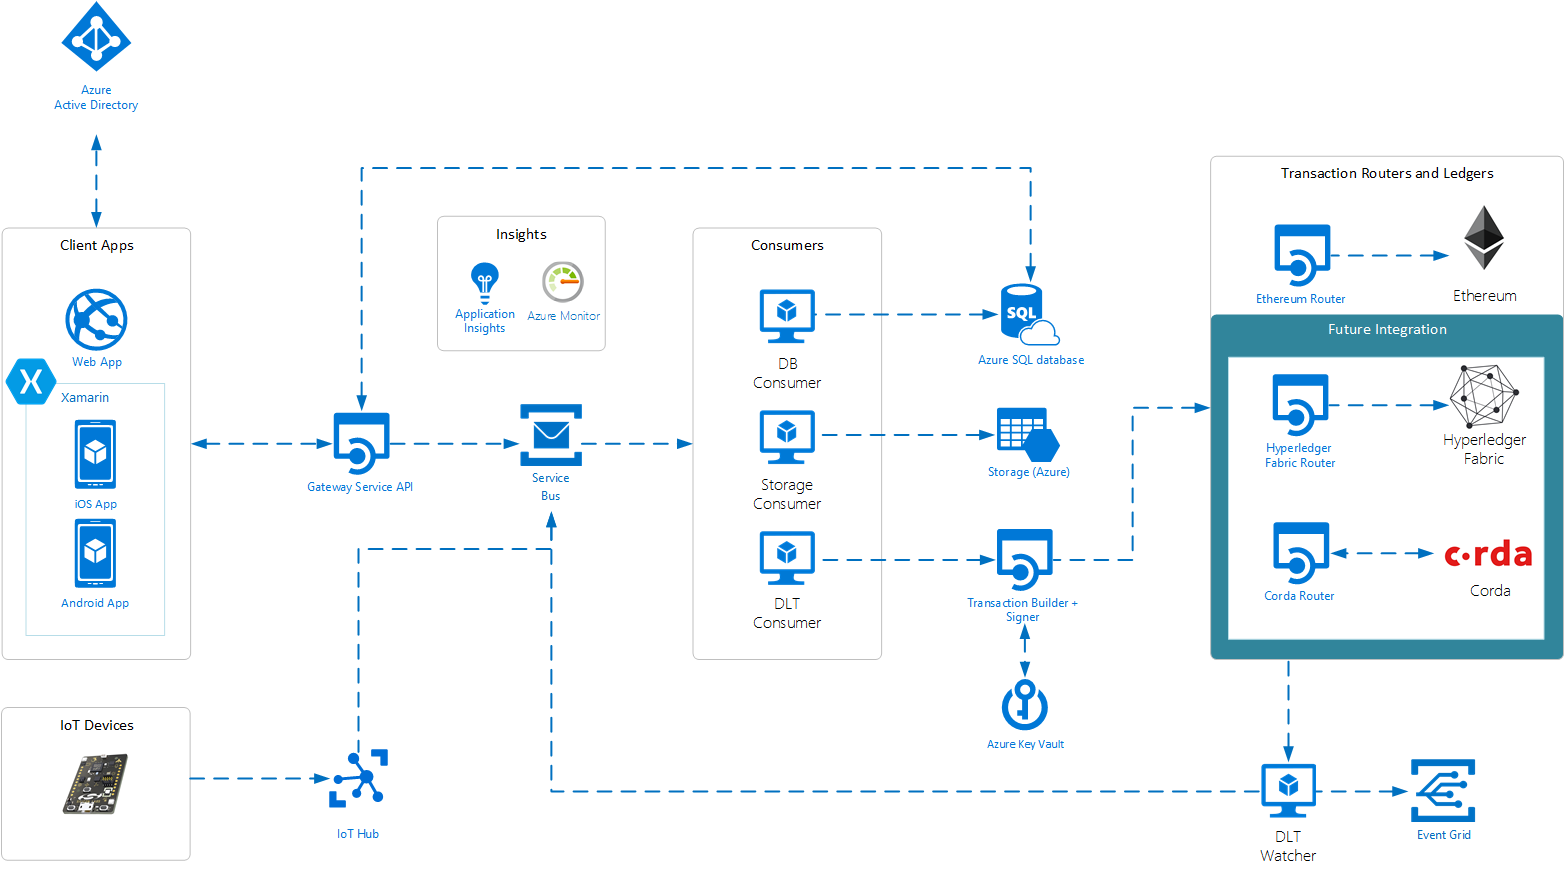
\includegraphics[width=0.75\textwidth]{figs/AZURE_architecture.png}
	\caption{Arquitecturas sugeridas por Azure para una estaci�n de Blockchain. Adaptado de \citep{AzureArchitectureSample}}\label{Arquitecturas sugeridas por Azure para una estaci�n de Blockchain}
\end{figure}

\begin{figure}[h]
	\centering
	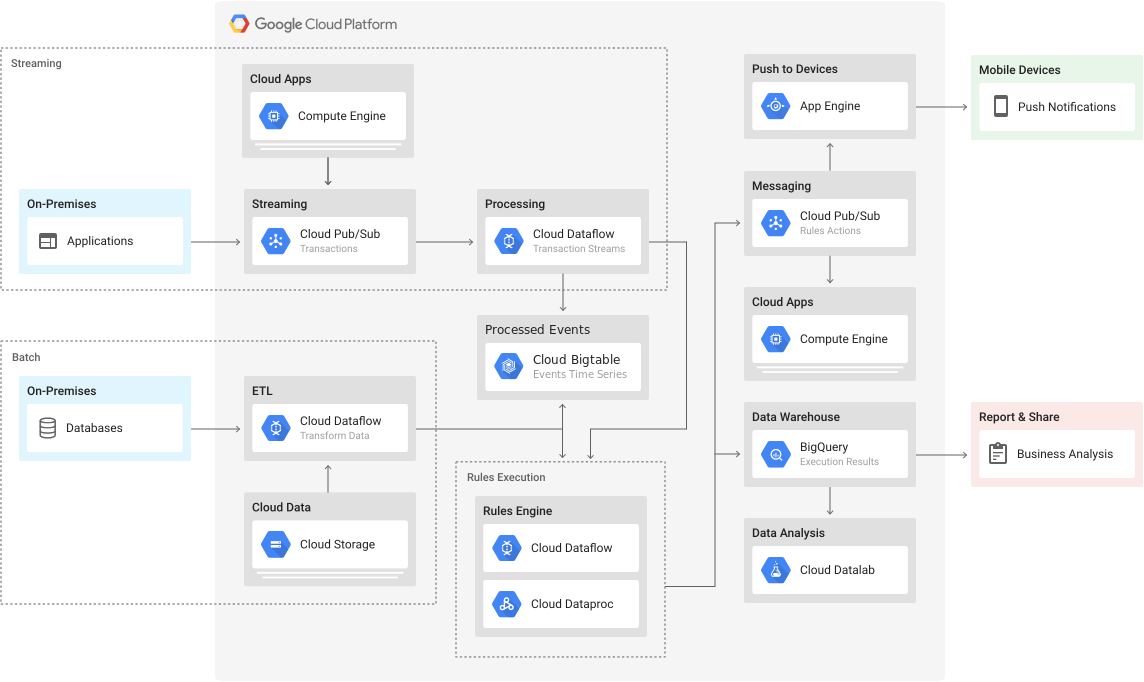
\includegraphics[width=\textwidth]{figs/GCP_architecture.png}
	\caption{Arquitecturas sugeridas por GCP para una aplicaci�n basada en eventos. Adaptado de \citep{GoogleArchitectureSample}}\label{Arquitecturas sugeridas por GCP para una aplicaci�n basada en eventos}
\end{figure}